\documentclass[notitlepage]{article}

\usepackage{bibunits}
\usepackage{comment}
\usepackage{graphicx}
\usepackage{amsmath}
\usepackage{amssymb}
\usepackage{datetime}
\usepackage{numprint}

% processes above options
\usepackage{palatino}  %OR newcent ncntrsbk helvet times palatino
\usepackage{url}
\usepackage{footmisc}
\usepackage{endnotes}
\usepackage{graphicx}
\graphicspath{{./hw1}}

\setcounter{secnumdepth}{3}
\begin{document}

\nplpadding{2}
\newdateformat{isodate}{
  \THEYEAR -\numprint{\THEMONTH}-\numprint{\THEDAY}}
  
\title{Homework 1}
\author{Esteban Calvo}
\date{\isodate\today}

\maketitle

\newpage


 \section*{Exercise 1}
    \textbf{Theorem}: z is real if and only if $\bar{z} = z$ \\
   \textbf{Proof}: \\
         
        Suppose for the sake of contradiction that z is a complex number in the form of 
        z = x + iy. By the definition of $\bar{z}$, $\bar{z} = x- iy$ and therefore, if z
        is a complex number, $\bar{z} \neq z$.\\

        Now, we must show that this works both ways and thus must show that if $\bar{z} = z$,
        then z is real. We can once again use the definition
        of $\bar{z}$ to be $\bar{z} = x-iy$. The definition of z is $z = x+iy$ and therefore, for
        $\bar{z} = z$, we must conclude that y is equal to 0 and therefore we are left with 
        $x = x$ and therefore know that z and $\bar{z}$ must both be real numbers.\\~\\
    \textbf{Theorem}: z is either real or pure imaginary if and only if $\bar{z}^2 = z^2$ \\
    \textbf{Proof}: \\

        Suppose for the sake of contradiction that z is neither real nor pure imaginary and is therefore
        a complex number in the form of z=x+iy. We also know the definition of $\bar{z}=x-iy$. From here,
        we can square both numbers and see that $z^2 = x^2-y^2+2ixy$ and $\bar{z}^2=x^2-y^2-2ixy$ 
        and therefore, z cannot be a complex number and is therefore either real or imaginary. \\

        Now, we must show that if $\bar{z}^2 = z^2$, then z is either real or imaginary. To begin,
        we can use the expanded out final equation $z^2 = x^2-y^2+2ixy$ and $\bar{z}^2=x^2-y^2-2ixy$.
        In this case, we can see that this is only the case if either x or y is zero such that we get
        $x^2-y^2 = x^2-y^2$. Since either is true, we know that z is either real (no y) or pure imaginary
        (no x) and therefore the proof is complete. \\~\\

 \section*{Exercise 2}

        \hspace{1cm} De Moivre's formula is as follows:
        $$(cos(\theta) + i*sin(\theta))^n=cos(n\theta)+i*sin(n\theta)$$
        In this case, we want n=3 and therefore can begin with the following equation:
        $$cos(3\theta)+i*sin(3\theta)$$
        and therefore can rewrite this into the following equation using De Movire's formula
        $$(cos(\theta)+i*sin(\theta))^3$$
        Expanding this out yields the following formula:
        $$cos^3(\theta)+3i*sin(\theta)cos^2(\theta)-3sin^2(\theta)cos(\theta)-isin^3(\theta)$$
        and now we can factor this out to the following:
        $$(cos^3(\theta)-3sin^3(\theta)cos(\theta)) + i(3sin(\theta)cos^2(\theta)-sin^3(\theta))$$
        
        At this point, we have found that $(cos(\theta)+i*sin(\theta))^n$ equals the formula above 
        and can therefore go back to the original formula of  $(cos(\theta) + i*sin(\theta))^n=cos(n\theta)+i*sin(n\theta)$
        and can therefore conclude that for the LHS to equal the RHS
        \begin{equation}
            \begin{aligned}
                & cos(3\theta) = cos^3(\theta)-3(\theta)sin^2(\theta)\notag\\
                &sin(3\theta) = 3cos^2(\theta)sin(\theta)-sin^3(\theta)
            \end{aligned}
        \end{equation}\\~\\

\section*{Exercise 3}

        \hspace{1cm} To begin, we can put the formula in the form of $z^4 = 1$. We can now use the definition of roots of unity
        which states that a root of unity is a complex number that when raised to a positive 
        integer power results in 1. The general form for a root of unity is as follows:
        $$z^n = 1 \ and\  e^{\frac{2k\pi*i}{n}}=C_k$$
        Where k is an integer such that k = 0,1,.., n-1 and n in this case is 4.
        So, using the roots of unity, we get that the 4 solutions are:
        $$1, e^{\frac{i\pi}{2}}, e^{i\pi}, e^{\frac{3i\pi}{2}}$$
        or we can eulers formula to further simplify this down to
        $$\pm 1, \pm i$$ \\~\\
        
\section*{Exercise 4}

    \hspace{1cm} To begin, we begin with the equation $\left| z - 1 - i \right| < 4$. We can use
    the definition of a modulus and expand this out to the equation $$\sqrt{(x-1)^2+(y-1)^2} < 4$$
    and therefore see that we are left with a circle that does not contain the border and is shifted 
    up and over 1 unit. This set is an open set as it does not contains it's border and all points
    inside of the circle U have a neighborhood\\
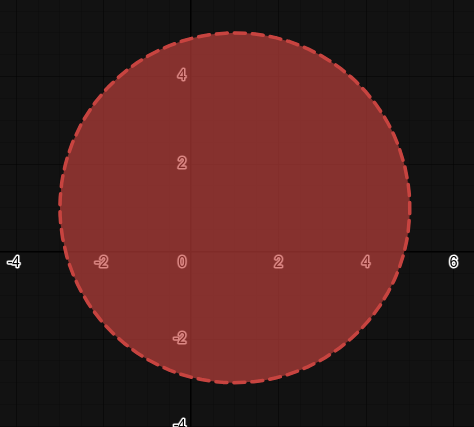
\includegraphics[scale=0.5]{hw1_4_1.png} \\
    We can use the same logic with $| z- 4 | \leq 3$ to get a circle that does contain the border and 
    is shifted over 4 units on the real axis.This set however is closed as it does contain its boundary
    and its complement is the open set of all points outside of the circle U.\\
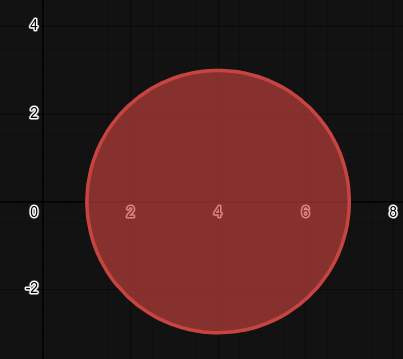
\includegraphics[scale=0.6]{hw1_4_2} \\
    Now, we have the equation $IM(z) > 1$ which is essentially asking for a graph such that $y > 1$
    and is therefore all imaginary parts that are greater than 1. This set is an open set as it does
    not contain the boundary y = 1\\
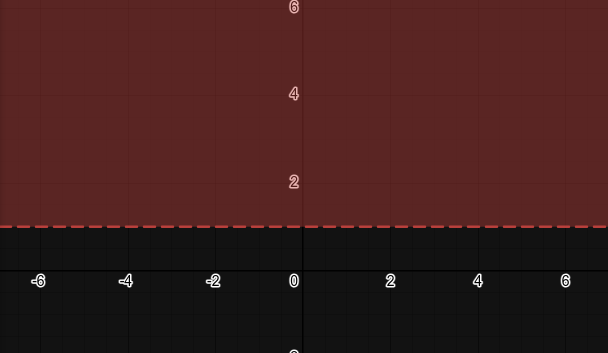
\includegraphics[scale=0.5]{hw1_4_3} \\
    Lastly, we have the same equation but with an equals instead. In this case, this is just a straight
    line along the value 1 on the imaginary axis. This set is a closed set as the graph is a line and is
    therefore impossible to find an open ball for any point on this line thus it cannot be an open set.\\
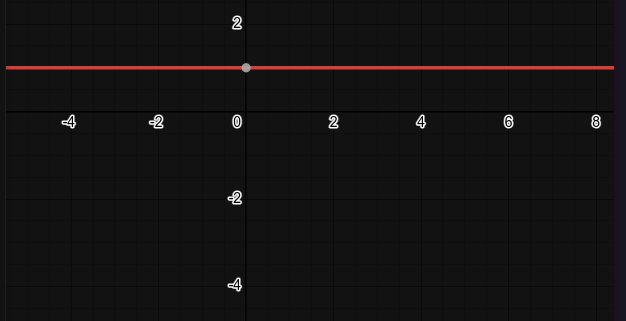
\includegraphics[scale=0.5]{hw1_4_4} \\~\\

\section*{Exercise 5}

    \hspace{1cm} We are asked prove that $|z| < 1$ and $|z-2| < 2$ are not connected. To do this,
    we can use the graph below. \\
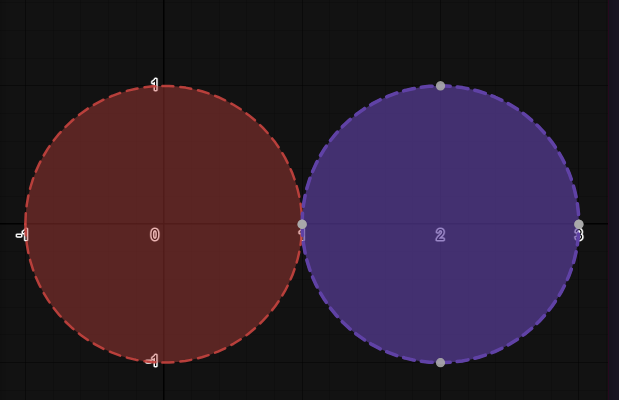
\includegraphics[scale=0.5]{hw1_5}\\
    From this graph, we can see that at x=2, the two borders meet. However, this point is not included
    in either of the two sets so if we were to take a point at $p_1=(0,0)$ and $p_2=(2,0)$, there is not a way 
    to get from $p_1$ to $p_2$. Thus, we have a disjointed set. \\~\\
    
\section*{Exercise 6}

    \hspace{1cm} To find the domain of definition for $f(z) = \frac{1}{z^2+1}$, we can set the denominator
    equal to 0 to see what points are excluded. Therefore, we have the equation $z^2+1=0$ and can rearrange
    this equation to get $z^2=-1$. Taking the square root on both sides gives that the denominator
    is 0 when $z=\pm i$. Therefore, the domain of definition can be expressed as 
    $$\{z \in C : z \neq \pm i \}$$ \\

    Now, we look at the equation $f(z) = z^6+z^3+100$. There is no point in this equation that can lead to
    to undefined behavior and therefore the domain of definition is
    $$\{ z \in C \}$$ \\~\\

\section*{Exercise 7}
    
    \hspace{1cm} To convert the equations from f(z) to terms of x and y, we an expand out the equations
    using the formula $z=x+iy$. To begin with the equation $f(z) = \frac{1}{z}$, we can first begin by 
    multiplying the equation $\frac{\bar{z}}{\bar{z}}$ which is equal to 1. In this case, $\bar{z} = x-iy$
    . Expanding out the equation to use x and y, we get
    \begin{equation}
        \begin{split}
            & \frac{1}{x+iy}*{\frac{x-iy}{i-iy}} \\
            & \frac{x-iy}{x^2+y^2} \\
            & \frac{x}{x^2+y^2}+\frac{-iy}{x^2+y^2} \notag
        \end{split}
    \end{equation}
and are therefore left with
\begin{equation}
    \begin{split}
        & u(x,y) = \frac{x}{x^2+y^2} \\
        & iv(x,y)= \frac{-y}{x^2+y^2} \notag
    \end{split}
\end{equation}\\

    Now, we move on the equation $f(z)=z^3+z+1$, we can expand this out and slowly group all the imaginary
    terms as follows
\begin{equation}
    \begin{split}
        f(z)&= (x+iy)^3 + (x+iy) + 1  \\
        &= (x^3+i3x^2y-3xy^2-iy^3)+(x+iy)+1\\
        &= (x^3-3xy^2+x+1)+i(3x^2y-y^3+y) \\
         \notag
    \end{split}
\end{equation}

and can therefore say
\begin{equation}
    \begin{split}
         \notag
        u(x,y)  &= x^3-3xy^2+x+1  \\
        iv(x,y) &=3x^2y-y^3+y \\
     \end{split}
\end{equation} \\~\\

\section*{Exercise 8}

    \hspace{1cm} To begin, we are given the definition of a limit is as follows: \\
     For each positive number $\epsilon$, there is a positive number $\delta$ such that
    $|f(z) - \omega_0|$ whenever $0 < |z-z_0| < \delta$ \\
    a) $\lim\limits_{z \to z_0}Re(z)=Re(z_0)$ \\
        To begin, we can consider $Re(z) = Re(x+iy) = x$ and therefore
\begin{equation}
    \begin{split}
        \omega_0    &= f(z_0) \notag\\
                    &= Re(z_0) \\
                    &= Re(x_0+iy_0) \\
                    &= x_0 \\
    \end{split}
\end{equation}
    From here, we can use both $f(z)$ and $f(z_0)$ as follows

\begin{equation}
    \begin{split}
        |f(z)-\omega_0|  &= |Re(z)-Re(z_0)| \notag\\
                         &= |x-x_0| \\
                         &= \sqrt{(x-x_0)^2} \\
                         &\leq \sqrt{(x-x_0)^2+(y-y_0)^2} \\
                         &= |z-z_0| < \delta \\
    \end{split}
\end{equation}
    and therefore $\lim\limits_{z \to z_0}Re(z)=Re(z_0)$ \\~\\
   b)  $\lim\limits_{z \to z_0}\bar{z}=\bar{z_0}$ \\
    We can use the definition of $\bar{z} = (x-iy)$ to and $\omega_0 = \bar{z_0}$ in this case
    to begin with the inequality $|\bar{z}-\bar{z_0}| < \epsilon$. We also have the inequality
    $0 < | z - z_0| < \delta$. If we expand both of these inequalities, we see that we have
\begin{equation}
    \begin{split}
            |\bar{z}-\bar{z_0}| = |(x-iy)-(x_0-iy_0)|  &= \sqrt{(x-x_0)^2+(y_0-y)^2} \\
            |z - z_0| = |(x+iy)-(x_0+iy_0)| &= \sqrt{(x-x_0)^2+(y-y_0)^2} \\
            \notag
    \end{split}
\end{equation}
    and thus we can see that they are both equal therefore this limit exists when $\delta = \epsilon$\\~\\
    c)  $\lim\limits_{z \to 0}\frac{\bar{z}^2}{z} = 0$ \\
    To begin, we can use some modulus properties and perform the following operations
\begin{equation}
    \begin{split}
        & |f(z)-0| < \epsilon \\
        & |\frac{\bar{z}^2}{z}-0| < \epsilon \\
        & \frac{|z|^2}{|z|}  < \epsilon \\
        & |z| < \epsilon \\
        \notag
    \end{split}
\end{equation}
    and we can once again choose $\epsilon=\delta$ and this limit will now hold as both inequalities are the same
    as we have $0 < |z| < \delta$ and $|z| < \epsilon$
\section*{Exercise 9}

    \hspace{1cm} We begin with the following given equation
    $$T(z) = \frac{az+b}{cz+d} \ (ad-bc) \neq 0$$ \\
    Theorems:\\
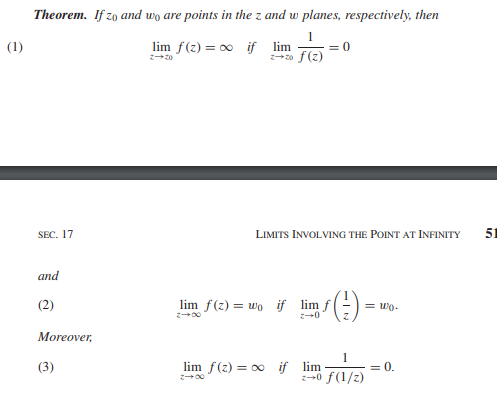
\includegraphics[scale=0.4]{hw1_9} \\
    a)  $\lim\limits_{z \to \infty}T(z) = \infty$ if $c=0$\\
    We can begin with theorem 3. So, we can begin to rewrite the equation as follows
\begin{equation}
    \begin{split}
        \notag
        \lim\limits_{z \to 0} \frac{1}{T(1/z)} &=  \lim\limits_{z \to 0} \frac{1}{T(z^{-1})} \\
                &=  \lim\limits_{z \to 0} \frac{1}{(\frac{az^{-1}+b}{cz^{-1}+d})} \\
                &=  \lim\limits_{z \to 0} \frac{cz^{-1}+b}{az^{-1}+b} * \frac{z}{z} \\
                &=  \lim\limits_{z \to 0} \frac{c+dz}{a+bz} \\
                &= \frac{c}{a} \ and \ c=0\\
                &= 0 \\
    \end{split}
\end{equation}
    Therefore, we have shown that the limit approaches infinity if c = 0 \\~\\
    b) $\lim\limits_{z \to \infty}T(z) =\frac{a}{c}$ and 
    $\lim\limits_{z \to -d/c}T(z) = \infty$ if $c\neq 0$  \\
    To begin, we can see that are using theorems 1 and 2 for this example and can begin with solving
    the first limit.
\begin{equation}
    \begin{split}
        \notag
         \lim\limits_{z \to \infty}T(z) &= \frac{a}{c} \\
                 &= \lim\limits_{z \to 0}T(1/z)\\
                 &=   \lim\limits_{z \to 0}(\frac{az^{-1}+b}{cz^{-1}+d})  * \frac{z}{z}\\
                 &= \lim\limits_{z \to 0}\frac{a+bz}{c+dz} \\
                 &= \frac{a}{c}
    \end{split}
\end{equation}
    We also need to show the second limit as follows
\begin{equation}
    \begin{split}
        \notag
        \lim\limits_{z \to -d/c}\frac{1}{T(z)} &= \lim\limits_{z \to -d/c}\frac{1}{(\frac{az+b}{cz+d})} \\
         &= \lim\limits_{z \to -d/c}\frac{cz+d}{az+b} \\
          &= \frac{c*(-d/c)+d}{a(-d/c)+b} \\
          &= \frac{-d+d}{a(-d/c)+b} \\
          &= \frac{0}{a(-d/c)+b}
  \end{split}
\end{equation}
    We are given that $ad-bc \neq 0$ which we can manipulate to be the equation 
    $a(d/c) - b \neq 0$. We can further manipulate this to be $-(a(-d/c)+b) \neq 0$ and therefore
    we know that the denominator above is not zero and can therefore reduce the fraction to be 
    $\frac{0}{\epsilon}$ such that $\epsilon \in \mathbb{R}$ and therefore zero. \\~\\

\section*{Exercise 10}

    a) $f(z) = 3z^2-2z+4$ \\
        We can use the formula $\frac{d}{dz}z^n = nz^{n-1}$ to get the final solution of
        $$f'(z) = 6z - 2$$
    b) $f(z) = (2z^2+i)^5$ \\
            For this problem, we can use the chain rule to get the following solution
\begin{equation}
    \begin{split}
        \notag
        f'(z) &= 5(2z^2+i)^4*(4z) \\
                &= 20z(2z^2+i)
    \end{split}
\end{equation}

    c) $f(z) = \frac{z-1}{2z+1} \ (z\neq -\frac{1}{2})$
    For this problem, we can use the quotient rule
 \begin{equation}
    \begin{split}
        f(z)    &= \frac{z-1}{2z+1} \\
        f'(z)   &= \frac{\frac{d}{dz}(z-1)(2z+1) - (z+1)\frac{d}{dz}(2z+1)}{(2z+1)^2} \\ 
                &= \frac{(2z+1)-2(z-1)}{(2z+1)^2} \\
                &= \frac{3}{(2z+1)^2}
        \notag
    \end{split}
\end{equation}


    d) $f(z) = \frac{(1+z^2)^4}{z^2} \ (z \neq 0)$
\begin{equation}
    \begin{split}
        \notag
        f'(z)   &= \frac{\frac{d}{dz}(1+z^2)^4(z^2) - (1+z^2)^4\frac{d}{dz}z^2}{z^4} \\
                &= \frac{4(1+z^2)^3(2z)(z^2) - (1+z^2)^4(2z)}{z^4} \\
                &= \frac{8z^2(1+z^2)^3-2(1+z^2)^4}{z^3} \\
                &= \frac{2(z^2+1)^3(3z^2-1)}{z^3}
    \end{split}
\end{equation}


\end{document}
